\chapter{BPM}\label{chp:bpm}

\section{Processos de Negócio}\label{sec:bpm-processos}
Um processo de negócio é definido por um conjunto de atividades coordenadas, relacionadas entre si, que envolvem diferentes pessoas, procedimentos, áreas e tecnologias com o objetivo de gerar valor para a empresa, seja em forma de produtos ou serviços, internos ou externos.

\section{BPM}\label{sec:bpm-bpm}
BPM\cite{bpm} é o acrônimo em inglês para \textit{Business Process Management}, ou em português \textit{Gerenciamento de Processos de Negócio}. Seu principal objetivo é oferecer uma abordagem sistemática para a execução, adaptação e melhoria de processos de negócio em um ambiente de constantes mudanças. 

Diferentemente de métodos tradicionais, que são focados no desempenho das unidades funcionais de uma empresa, a adoção do BPM como disciplina de gestão concentra-se no controle e melhoria contínua dos processos funcionais que, na maioria das vezes, permeiam diferentes áreas de negócio.

A aplicação do BPM não deve necessariamente envolver tecnologia. Na prática, diversas melhorias de processos podem ser alcançadas sem a utilização de tecnologia ou sistemas de informação. Por exemplo, através da análise e mapeamento de processos de logística, muitas vezes é possível implementar melhorias no processo através do sequenciamento otimizado das tarefas que o constituem, implicando em menos tempo despendido para sua execução.

Entretanto, quando avaliamos a aplicação de BPM em processos críticos, complexos ou até mesmo processos simples mas executados em maior escala, a aplicação de tecnologia torna-se fundamental. A melhoria e automatização de processos através da aplicação de tecnologia é comumente vista na utilização de sistemas de informação para suportar a execução de diferentes tipos de processos, como ocorre normalmente um CSC\cite{csc} (Centro de Serviços Compartilhados).


\section{BPMN}\label{sec:bpm-bpmn}
BPMN\cite{bpmn} é o acrônimo em inglês para \textit{Business Process Management Notation}, ou em português \textit{Notação de Gerenciamento de Processos de Negócio}. Foi criada para representar processos de negócio em forma de diagrama, através de uma notação padronizada e de fácil entendimento por diferentes profissionais, sejam eles desenvolvedores, analistas de negócio ou gestores. Foi criada inicialmente pelo BPMI\cite{bpmi} (Business Process Management Initiative) em 2004, entretanto é mantida atualmente pela OMG\cite{omg} (Object Management Group). Sua versão mais atual é a BPMN 2.0\cite{bpmn20}, publicada em 2011.

A notação foi concebida sob a perspectiva de cobrir a falta de entendimento entre diferentes departamentos e organizações a cerca de um determinado processo ou conjunto de processos, algo muito frequente no ambiente corporativo. Além disso, através de sua notação padronizada em XML\cite{xml} (Extensible Markup Language), diferentes ferramentas podem fazer o uso de sua auto-descrição para informatizar a orquestração de processos de negócio.



\begin{figure}[H]
  \centering
  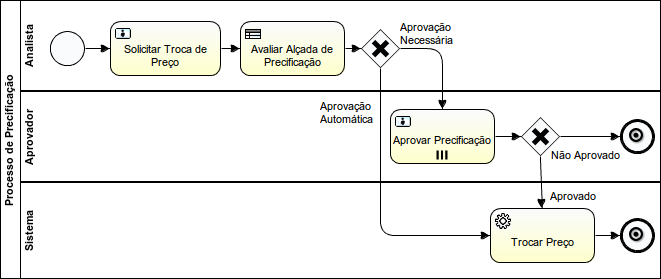
\includegraphics[width=1.0\textwidth]{imagens/ProcessoDePrecificacao.png}
  \caption{Processo representado em BPMN}
  \label{fig:exemplo_bpmn}
\end{figure}

A figura \ref{fig:exemplo_bpmn} mostra um exemplo de processo modelado na ferramenta Activiti Designer que será abordada em mais detalhes no capítulo \ref{chp:activiti-bpm} e representa o cenário descrito na seção \ref{sec:problema-exemplo}. Os elementos do modelo serão explicados ao longo deste capítulo.


\subsection{Objetos}\label{sec:bpm-bpmn_objetos}

A notação define quatro grupos distintos de objetos para permitir a diagramação de um fluxo de negócio. Os objetos são classificados em artefatos, agrupadores, conectores e objetos de fluxo. São utilizadas figuras geométricas, como retângulos e círculos, além de linhas pontilhadas e tracejadas, entre outros elementos gráficos para representar cada um dos objetos que constituem a notação.

\subsubsection{Objetos de Fluxo}\label{sec:bpm-bpmn_objetos_fluxo}

Os objetos de fluxo são os principais elementos do BPMN pois constituem os elementos chave na execução do fluxo de trabalho. Eles são dividos em 3 principais grupos que serão detalhados a seguir: eventos, atividades e decisões.


\begin{enumerate}
    \item Eventos
    
    Objetos utilizados para representar que algo "aconteceu" durante a execução do fluxo. São exemplos de eventos: "chamada de sistema externo recebida", "envio de cancelamento do processo recebido", "a cada 1 minuto". A notação BPMN 2.0 define mais de 60 tipos distintos de eventos. A figura \ref{fig:bpmn_events} mostra os diferentes tipos de eventos e suas notações.
    
    \begin{figure}[H]
    \centering
    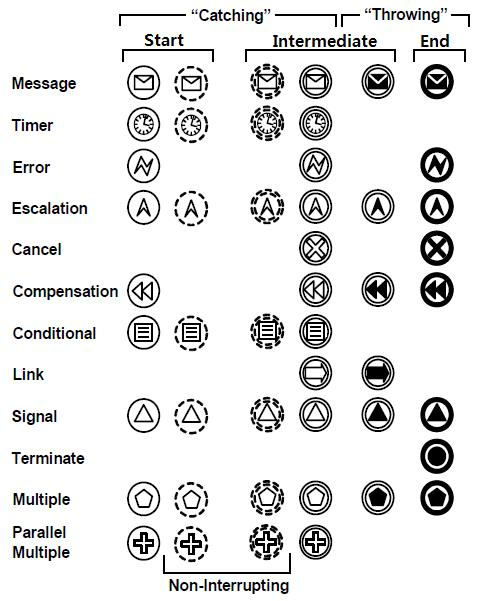
\includegraphics[width=0.65\textwidth]{imagens/bpmn_events.jpg}
    \caption{Tipos de Eventos}
    \label{fig:bpmn_events}
    \end{figure}
    
    Na figura, os elementos estão divididos de acordo com o momento do processo em que podem ocorrer: início -- são os eventos que podem criar uma nova instância de processo, intermediários -- são os eventos que ocorrem durante a execução do processo, e finais -- são os eventos que indicam fim do processo, seja ele por sucesso ou erro.
    
    \item Atividades
    
    Objetos utilizados para representar uma unidade de trabalho a ser realizada no processo. Existem dois tipos básicos de atividades: tarefas ou subprocessos. As tarefas podem ser executadas por humanos ou por algum tipo de serviço, como um seviço web ou mesmo a execução de algum código interno no processo. Já os subprocessos são atividades utilizadas para agrupar outros objetos, encapsulando fluxos de maior complexidade.
    
    \begin{figure}[H]
    \centering
    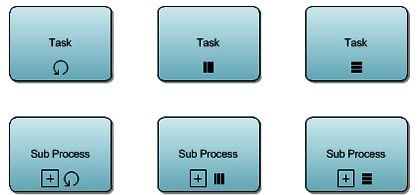
\includegraphics[width=0.55\textwidth]{imagens/bpmn_activities.jpg}
    \caption{Tipos de Atividades}
    \label{fig:bpmn_activities}
    \end{figure}
    
    A mesma atividade pode ser executada uma ou mais vezes, e a figura \ref{fig:bpmn_activities} mostra as notações utilizadas para indicar multiplicidade. A seta circular nas atividades mais à esquerda, indica que estas atividades serão executadas até determinada condição ser satisfeita. Já as linhas paralelas, nas outras atividades da figura, indicam execuções múltiplas, iterando em cada item de uma coleção previamente definida no processo. As linhas verticais representam que essa iteração ocorre paralelamente, ou seja, cada uma das instâncias da atividade ocorre concomitantemente e sem ordem de execução definida. Já as linhas horizontais significam que a execução das atividades é sequencial, onde uma só será iniciada após o término da anterior.
    
    \item Decisões
    
    São objetos utilizados para controlar o fluxo de trabalho, possibilitando o direcionamento do processo para a escolha de único sentido, ou para controlar a divergência e convergência de fluxos paralelos. Essas decisões podem ser feitas com base nos dados inerentes ao fluxo do processo ou em eventos relacionados à sua execução.
    
    \begin{figure}[H]
    \centering
    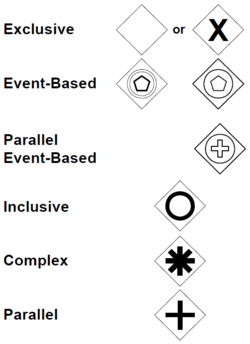
\includegraphics[width=0.4\textwidth]{imagens/bpmn_gateways.png}
    \caption{Tipos de Decisões}
    \label{fig:bpmn_gateways}
    \end{figure}
\end{enumerate}

    A figura \ref{fig:bpmn_gateways} mostra a notação dos diferentes tipos de decisões que podem ser aplicadas ao contexto de um projeto. Elas podem ser exclusivas (apenas um fluxo é seguido, notações exibidas na primeira linha), inclusivas (um ou mais fluxos podem ser executados, notação mostrada na quarta linha), paralelas (todos os fluxos são executados de maneira independente, notação exibida na última linha) e baseadas em eventos, em vez de dados do processo, que também podem ser exclusivas, como as notações da segunda linha, ou paralelas, como as da terceira linha.


\subsubsection{Agrupadores}\label{sec:bpm-bpmn_objetos_agrupadores}

    São objetos utilizados para organizar visualmente a distribuição dos demais objetos do processo em contêineres que representam a responsabilidade de determinado ator do processo.

    \begin{figure}[H]
    \centering
    
\includegraphics[width=0.5\textwidth]{imagens/bpmn_swimlanes.jpg}
    \caption{Tipos de Agrupadores}
    \label{fig:bpmn_swimlanes}
    \end{figure}
    
    A figura \ref{fig:bpmn_swimlanes} mostra os dois tipos de elementos utilizados para esta finalidade. \textit{Lane} é usada para agrupar tarefas do mesmo usuário, ou grupo de usuários que possuem as mesmas responsabilidades dentro de um processo, já a \textit{pool} é utilizada para agregar as diferentes \textit{lanes} do processo. 

\subsubsection{Artefatos}\label{sec:bpm-bpmn_objetos_artefatos}

    São utilizados para acrescentar informações adicionais a modelagem do processo. 

    \begin{figure}[H]
    \centering
    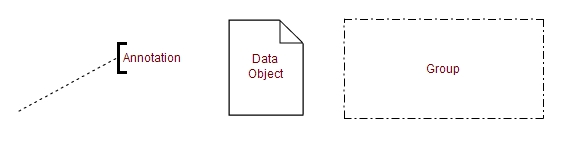
\includegraphics[width=0.8\textwidth]{imagens/bpmn_artifacts.jpg}
    \caption{Tipos de Artefatos}
    \label{fig:bpmn_artifacts}
    \end{figure}
    
    A figura \ref{fig:bpmn_artifacts} exemplifica os diferentes tipos de artefato. O primeiro são as anotações, usadas para adicionar comentários e/ou informações adicionais para facilitar o entendimento do processo, não possui nenhuma influência na execução do fluxo. O segundo é o objeto de dados, que serve para definir dados inerentes a execução do processo, que podem ser usados e manipulados pelos objetos de fluxo, por exemplo, servindo como critério para os objetos de decisão apresentados na seção \ref{sec:bpm-bpmn_objetos}. E o terceiro é o grupo, um retângulo utilizado para englobar objetos de fluxo de forma a a melhorar a organização do modelo -- assim como as anotações, possui apenas caráter visual, auxiliando a compreensão do processo através de recursos gráficos.


\subsubsection{Conectores}\label{sec:bpm-bpmn_objetos_conectores}

    São utilizados para interligar objetos de fluxo. São classificados em conectores de sequência, mensagem ou associação.

    \begin{figure}[H]
    \centering
    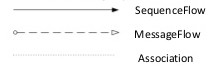
\includegraphics[width=0.5\textwidth]{imagens/bpmn_connectors.jpg}
    \caption{Tipos de Conectores}
    \label{fig:bpmn_conectors}
    \end{figure}
    
    A figura \ref{fig:bpmn_conectors} mostra a notação utilizada para os três diferentes tipos de conectores. O primeiro é o conector de sequência, que liga os objetos de fluxo, determinando a ordem de execução de cada um deles. O segundo é o conector de mensagem, que indica quando há troca de mensagens entre diferentes atividades, como uma chamada a um serviço \textit{web}, por exemplo. E, por último, a associação simples, que serve para relacionar logicamente diferentes elementos do modelo, mas não altera a execução do fluxo, por exemplo, relacionando um comentário a uma tarefa. 


\section{BPMS}\label{sec:automatizacao-processos-bpms}

BPMS\cite{bpms} é o acrônimo em inglês para \textit{Business Process Management Suites/System}, ou em português \textit{Sistemas de Gerenciamento de Processos de Negócio}. Os softwares BPMS são sistemas especialistas na modelagem, execução, controle e monitoramento de processos de negócio. 

A notação BPMN é geralmente utilizada para a modelagem dos processos, e interpretada pelo motor do BPMS que a utiliza para orquestração do fluxo de trabalho. Devido a sua abordagem focada em processos modelados por uma notação padronizada, o entendimento à cerca de um processo de negócio entre analistas de negócio e desenvolvedores acaba sendo facilitado. 

Dentre algumas das vantagens obtidas pelas organizações através da adoção de sistemas BPMS, podemos citar melhorias na capacidade de gestão e monitoramento de processos, melhorias na visibilidade e entendimento de processos, e maior rapidez na introdução de mudanças e ajustes nos processos de negócio.

Entre alguns fatores que diferenciam e caracterizam os sistemas BPMS, podemos citar o poder de automação promovido pela modelagem suportada, a possibilidade e facilidade de integração com demais sistemas de informação, a capacidade de análise, monitoramento e controle de processos e a interface do usuário com as atividades do processo.

Ao inspecionarmos o ecossistema de aplicações BPMS, podemos encontrar diversas opções variando desde soluções caríssimas até soluções gratuitas e de código-fonte aberto. Como exemplo de soluções pagas, podemos citar o SAP NetWeaver BPM\cite{bpm_sap} e Oracle BPM\cite{bpm_oracle}. Como exemplo de soluções com versões gratuitas ou de código-fonte aberto, podemos citar o Activiti BPM\cite{bpm_activiti}, Bonita BPM\cite{bpm_bonita} e Intalio BPM\cite{bpm_intalio}.

A maioria das aplicações BPMS mais robustas oferecem algum tipo de portal com o usuário, onde a interações humanas com os processos ocorrem. Neste portal, o usuário pode interagir com os processos, atuar em tarefas a ele designadas, iniciar ou cancelar processos, entre outras possibilidades de interação.

Da mesma forma que o portal, a maioria das ferramentas BPMS também oferece algum tipo de API. Isso abre a possibilidade de utilização de novas interfaces com o usuário e integração com outros sistemas. Isso possibilita a extensão do BPMS para outras plataformas não tradicionais em ambientes corporativos, como os dispositivos móveis ou até mesmo sensores, ou mesmo a customização de um novo portal que atenda as necessidades da corporação.


